% Vision, Color and Perception. Build with Tectonic or lualatex.
\documentclass[aspectratio=169,11pt]{beamer}

\usepackage{amsmath}
\usepackage{booktabs}
\usepackage{graphicx}
\usepackage{fontspec}
\usepackage{tikz}
\graphicspath{{figs/}}

% ---- UTS look shared with Seeing Data and Choosing Visual Forms ----
\setsansfont{Arial}
\definecolor{utsblue}{HTML}{0F4BEB}
\definecolor{utsred}{HTML}{FF2305}
\definecolor{utscyan}{HTML}{00B7E0}
\definecolor{utspale}{HTML}{C8D4F8}
\definecolor{ink}{HTML}{0A0A0A}
\definecolor{ground}{HTML}{FFFFFF}
\definecolor{mist}{HTML}{5A5F63}
\definecolor{scone}{HTML}{5B4BCE}
\definecolor{mcone}{HTML}{00A878}
\definecolor{lcone}{HTML}{E44B35}

\usetheme{default}
\renewcommand{\familydefault}{\sfdefault}
\setbeamertemplate{navigation symbols}{}
\setbeamercolor{background canvas}{bg=ground}
\setbeamercolor{normal text}{fg=ink}
\setbeamercolor{frametitle}{fg=ink}
\setbeamercolor{structure}{fg=utsblue}
\setbeamercolor{alerted text}{fg=utsred}
\setbeamertemplate{itemize item}{\color{utsred}\rule[0.45ex]{0.6em}{0.12em}}
\setbeamertemplate{itemize subitem}{\color{mist}\rule[0.45ex]{0.4em}{0.12em}}
\setbeamertemplate{frametitle}{%
  \vspace*{1.2em}%
  {\LARGE\bfseries\insertframetitle}\\[0.2em]
  {\color{utsred}\rule{3em}{0.18em}}%
}
\setbeamertemplate{footline}{%
  \hspace*{1.5em}{\color{mist}\tiny 36104 · Vision, Color and Perception}\hfill
  {\color{mist}\tiny UTS CRICOS 00099F · TEQSA PRV12060}\hfill
  {\color{mist}\tiny\insertframenumber}\hspace*{1.5em}\vspace*{0.8em}}

\colorlet{creditcolor}{mist}
\newcommand{\credit}[1]{{\color{creditcolor}\tiny #1}}
\newcommand{\kicker}[2]{%
  \begingroup
  \setbeamercolor{background canvas}{bg=utsblue}
  \setbeamercolor{normal text}{fg=white}
  \colorlet{creditcolor}{utspale}
  \begin{frame}[plain]
    \color{white}%
    \vspace*{0.9em}\noindent\hspace*{1.2em}%
    
\includegraphics[height=2.0em]{uts-logo-white.png}\par
    \begin{center}
      \vspace*{\fill}
      {\color{utspale}\bfseries\scriptsize\MakeUppercase{#1}}\\[0.6em]
      {\Huge\bfseries #2}
      \vspace*{\fill}
    \end{center}
  \end{frame}
  \endgroup}

\title{Vision, Color and Perception}
\author{36104 Data Visualisation and Narratives}

\begin{document}

% ---------- shared course cover ----------
\begin{frame}[plain]
  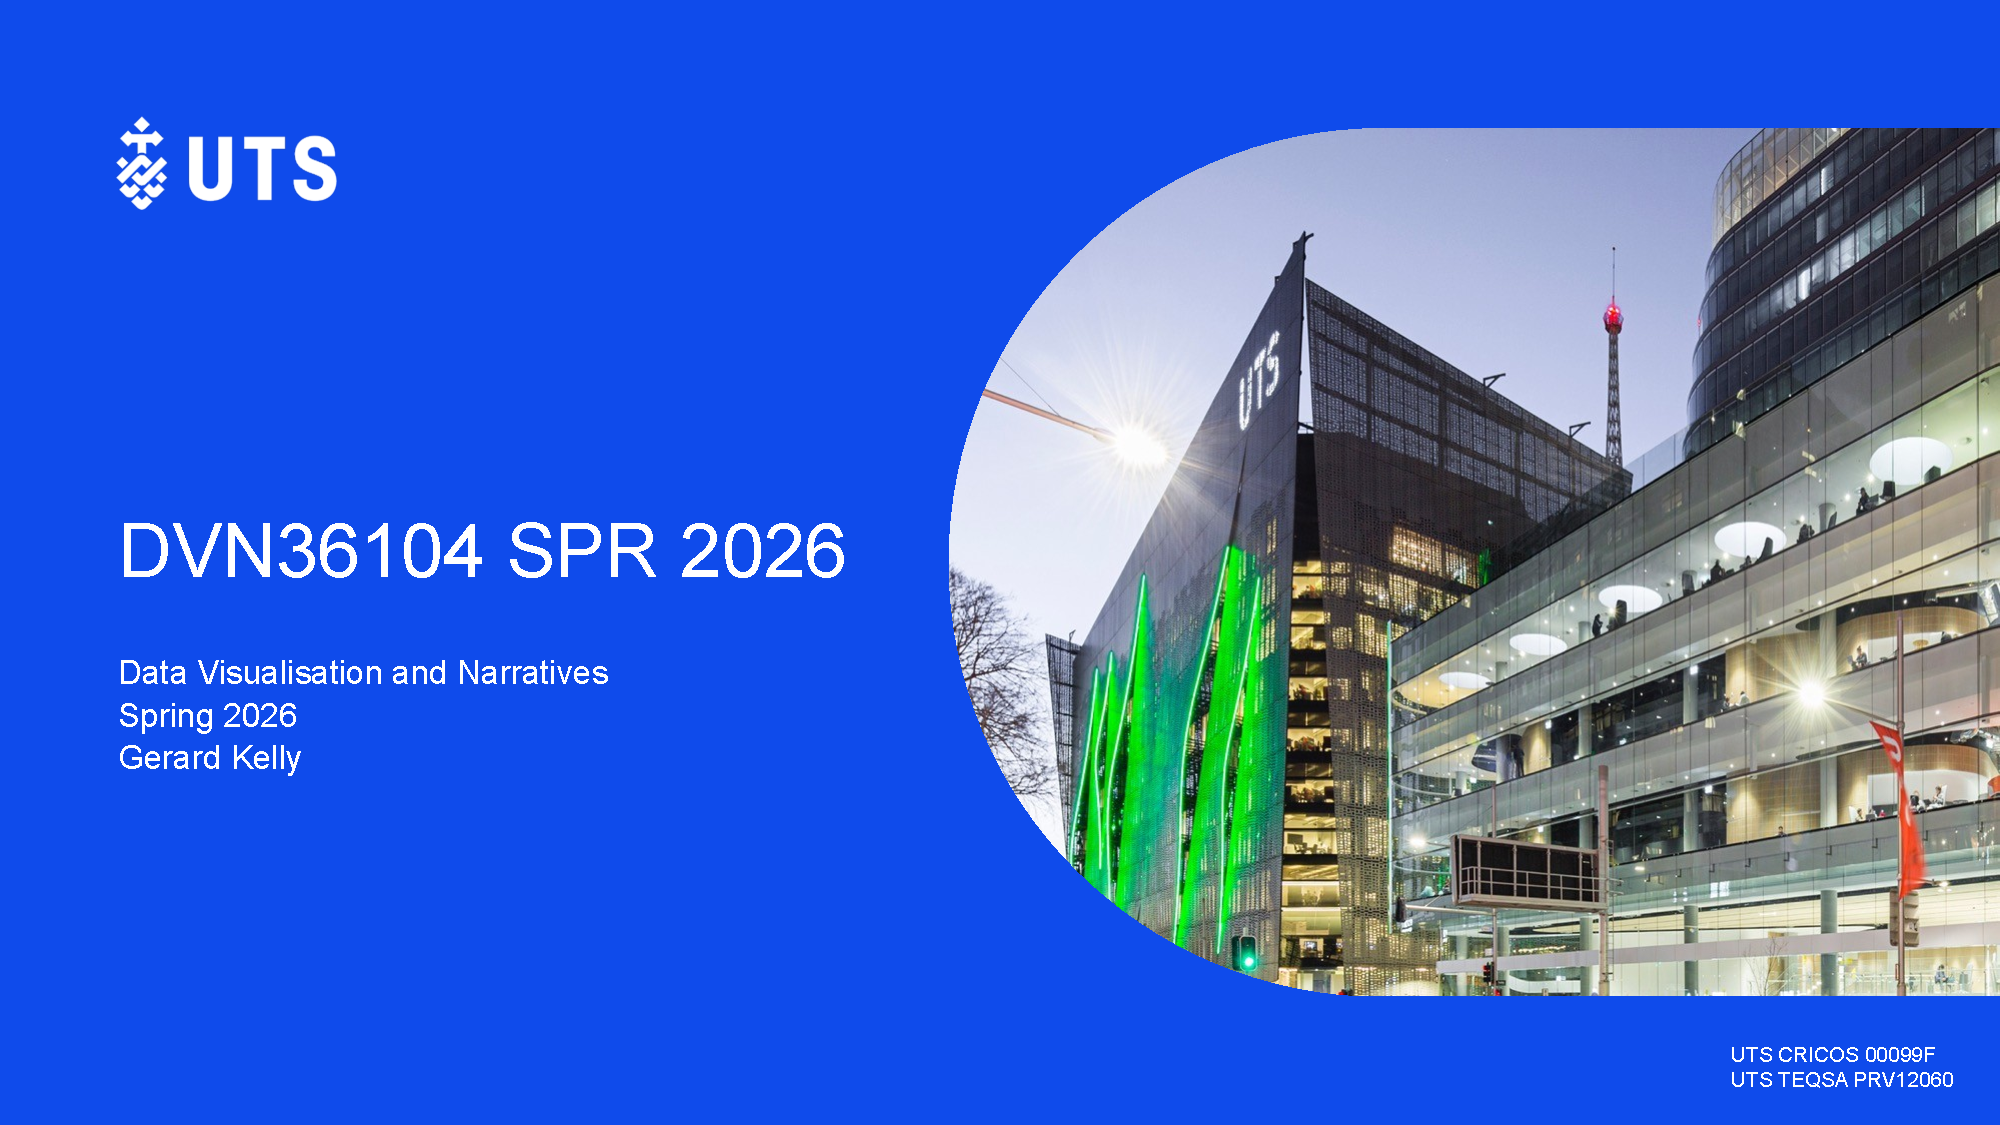
\includegraphics[width=\paperwidth,height=\paperheight]{../../../../cover.pdf}
\end{frame}

% ---------- topic title ----------
\begingroup
\setbeamercolor{background canvas}{bg=utsblue}
\setbeamercolor{normal text}{fg=white}
\begin{frame}[plain]
  \color{white}%
  \vspace*{0.9em}\noindent\hspace*{1.2em}%
  
\includegraphics[height=2.0em]{uts-logo-white.png}\par
  \vspace*{\fill}
  \hspace*{1.2em}{\color{utspale}\bfseries\scriptsize 36104 · DATA VISUALISATION AND NARRATIVES}\\[0.6em]
  \hspace*{1.2em}{\fontsize{34}{38}\selectfont\bfseries Vision, Color and Perception}\\[0.5em]
  \hspace*{1.2em}{\Large\color{utspale} Light, eyes, measurement, and screens}\\[2em]
  \hspace*{1.2em}{\small What survives as colour moves from the world into a visualisation?}
  \vspace*{\fill}
\end{frame}
\endgroup

\begin{frame}{One word, several different things}
  \small
  \begin{tabular}{@{}p{0.25\textwidth}p{0.66\textwidth}@{}}
    \toprule
    \textbf{When we say ``yellow''} & \textbf{we might mean} \\
    \midrule
    spectral light & power concentrated near one wavelength \\
    paint or flower & a surface reflectance under an illuminant \\
    appearance & an observer's experience in a context \\
    CIE coordinate & a standard-observer colour match \\
    screen colour & a coded request to three device primaries \\
    category & a word used by a community for a region of appearances \\
    \bottomrule
  \end{tabular}
  \vspace{0.7em}

  These descriptions can refer to related cases. They are not synonyms.
\end{frame}

\begin{frame}{Goals}
  \begin{enumerate}
    \item Distinguish wavelength, spectrum, cone response, appearance, coordinate, and code.
    \item Explain univariance and metamerism without the ``three colour buckets'' overclaim.
    \item Construct and read the CIE 1931 xy diagram.
    \item Explain why a three-primary display has a triangular gamut.
    \item Turn the model into a small Streamlit application.
  \end{enumerate}
\end{frame}

\kicker{Part I}{Start with the light}

\begin{frame}[t]{A wavelength is not a complete description of a light}
  \centering
  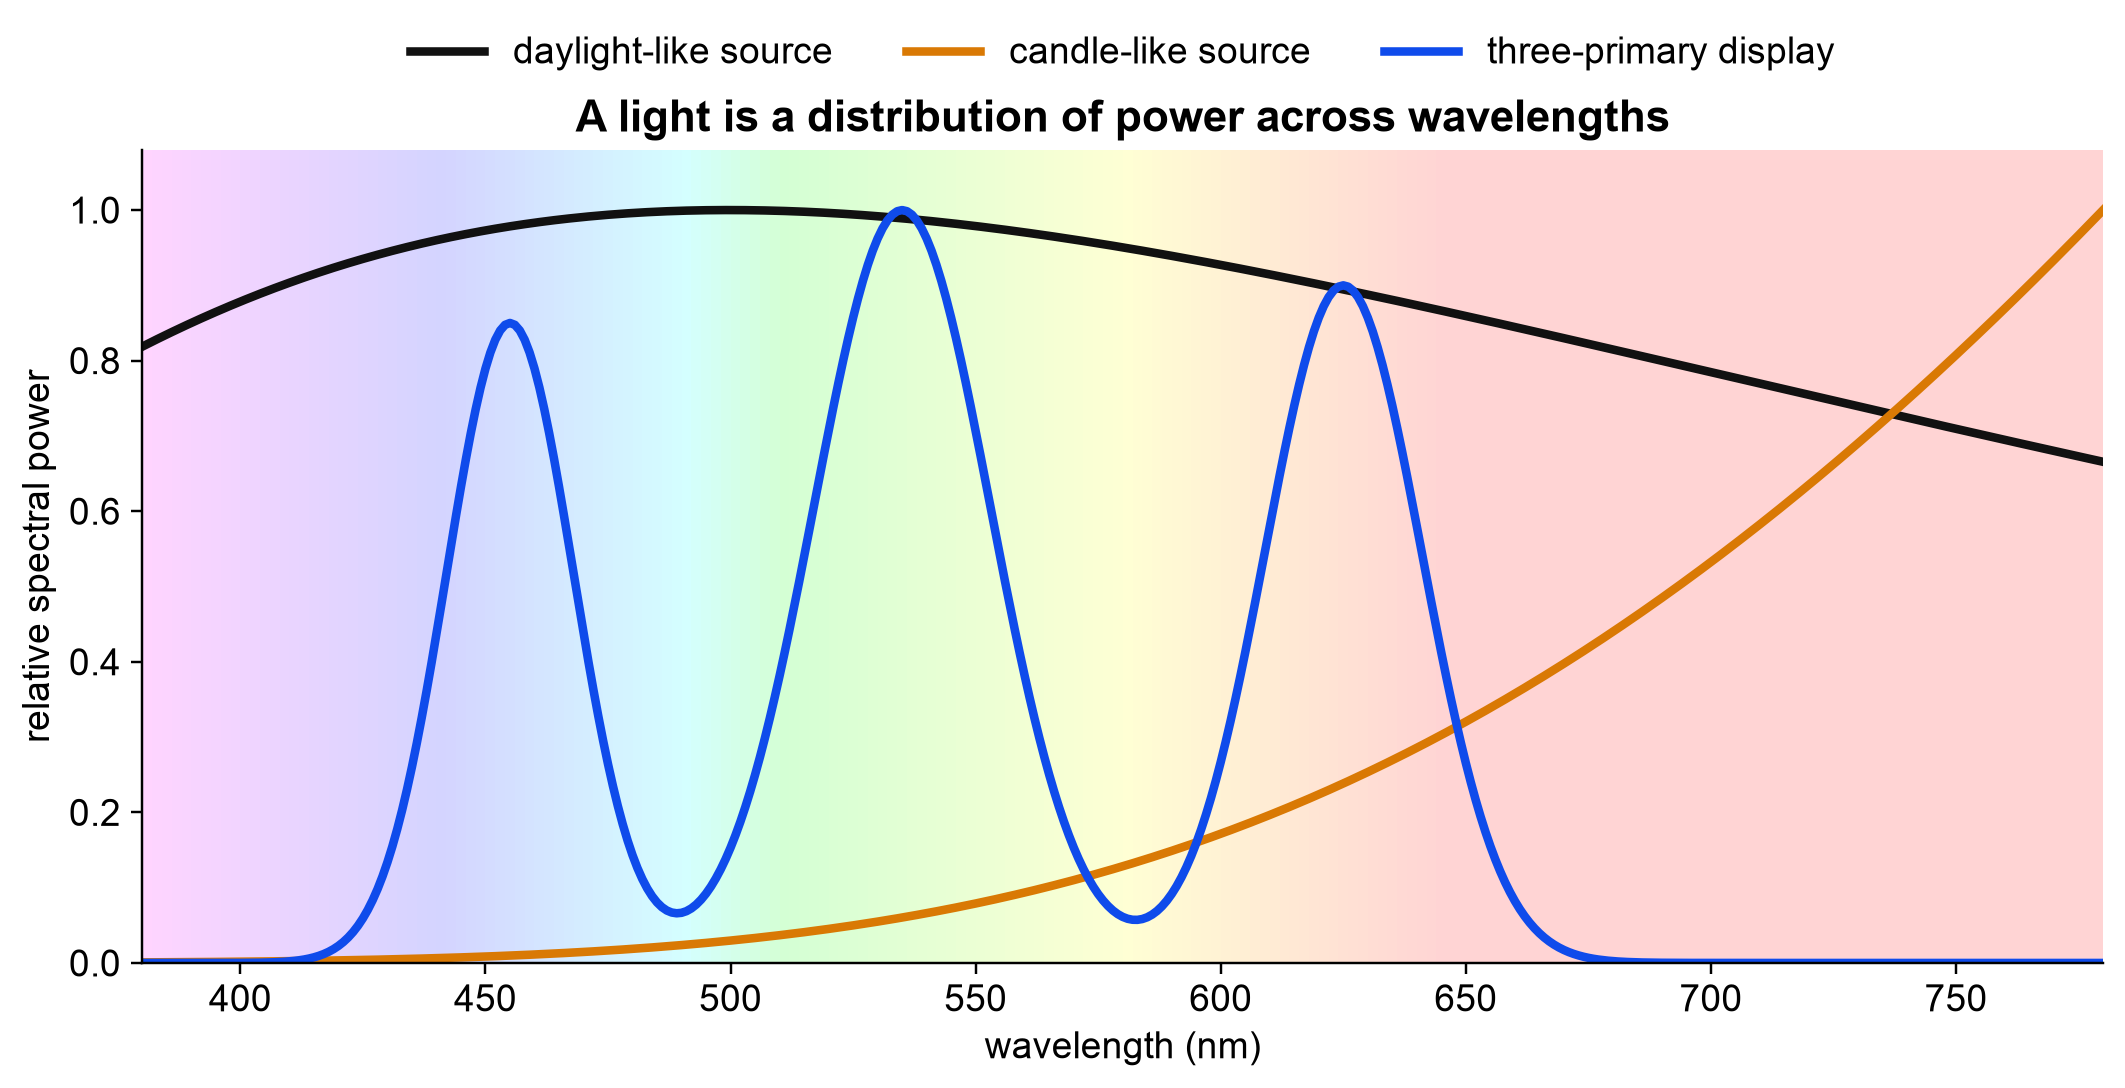
\includegraphics[width=0.88\textwidth,height=0.59\textheight,keepaspectratio]{fig-spectral-recipes.png}\\[-0.1em]
  \credit{Course calculation. Black-body curves are illustrative; display peaks are schematic.}
\end{frame}

\begin{frame}{A light is a function}
  \begin{columns}[T]
    \begin{column}{0.56\textwidth}
      \Large
      \[
        P(\lambda)=\text{power at wavelength }\lambda
      \]
      \normalsize
      A spectral power distribution contains one value for every wavelength sampled.
    \end{column}
    \begin{column}{0.39\textwidth}
      \small
      \begin{itemize}
        \item a narrow peak: approximately monochromatic;
        \item a broad curve: many wavelengths;
        \item three peaks: a typical display mixture;
        \item one colour word: none of the above is specified.
      \end{itemize}
    \end{column}
  \end{columns}
  \vspace{0.7em}
  \alert{The spectrum is the physical input. Colour appearance is a result downstream.}
\end{frame}

\begin{frame}[t]{An object does not send a fixed colour signal}
  \centering
  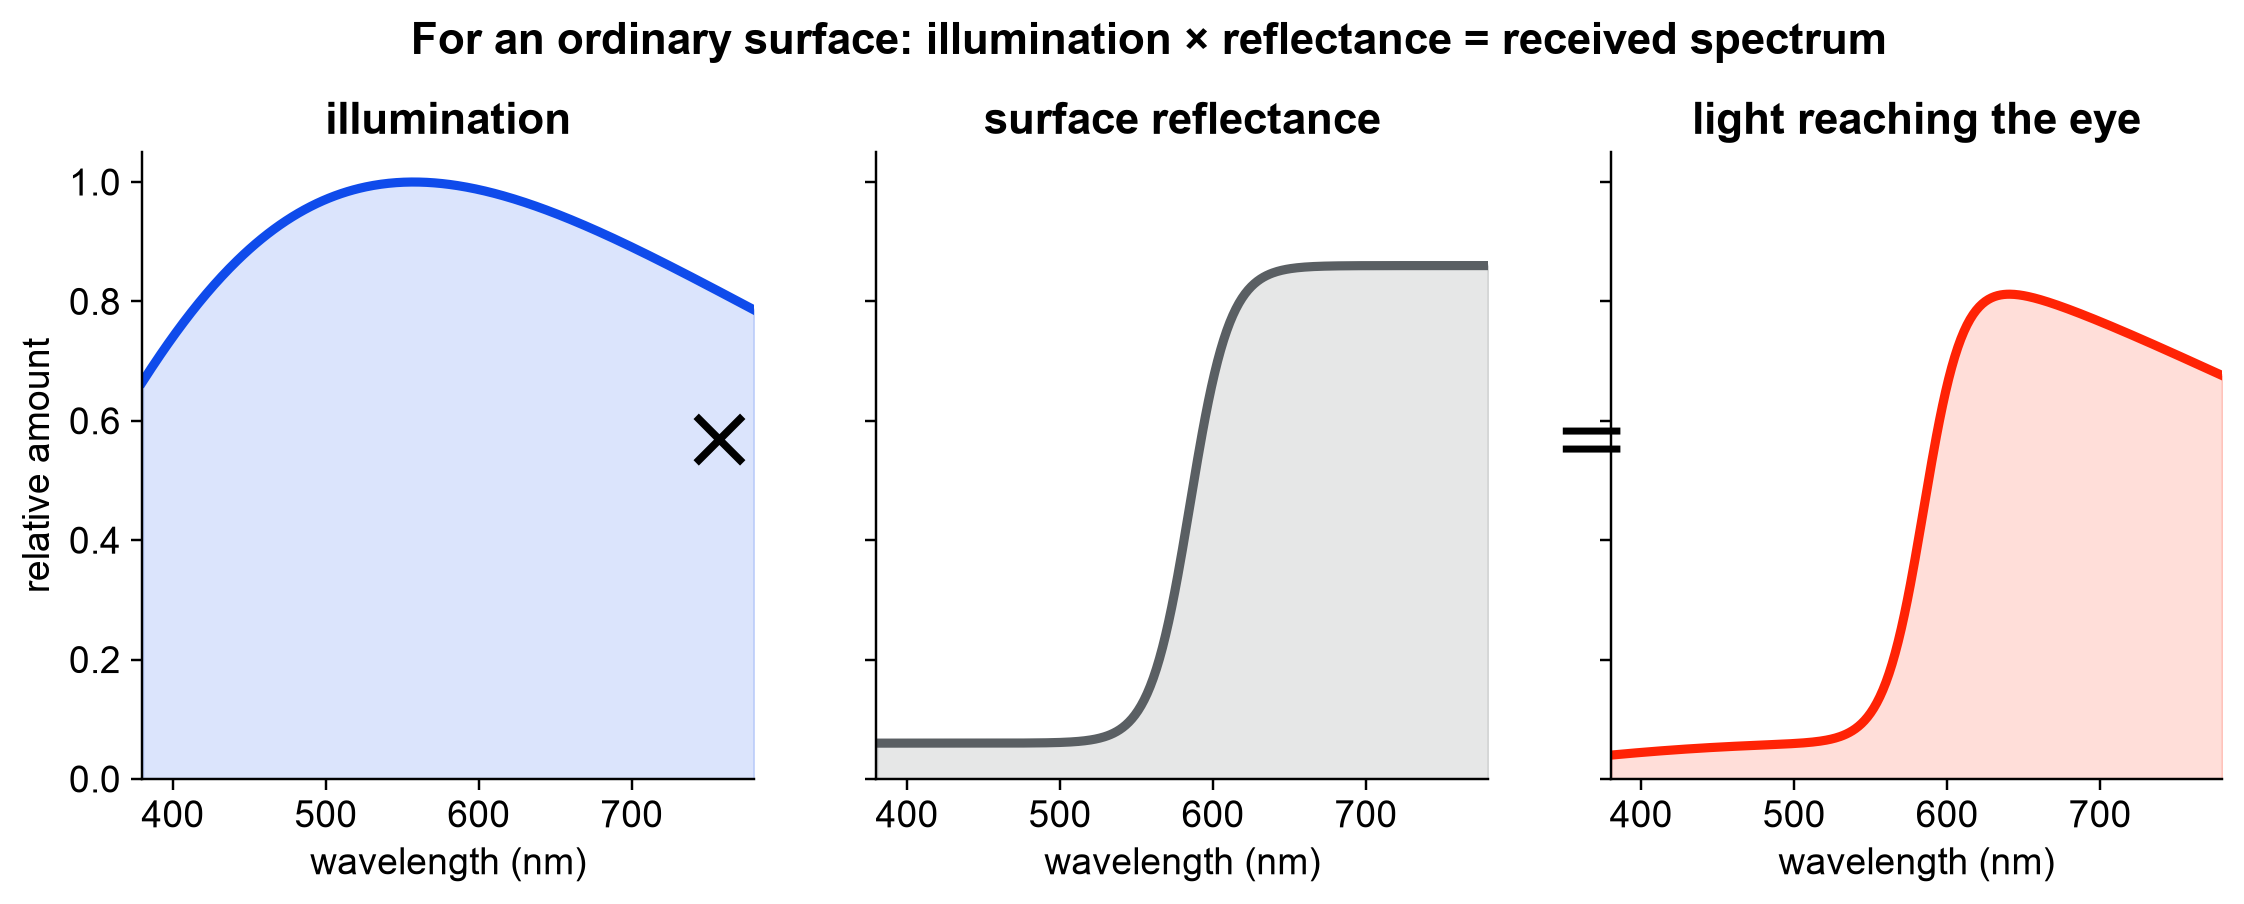
\includegraphics[width=0.94\textwidth,height=0.62\textheight,keepaspectratio]{fig-illumination-reflectance.png}\\[-0.1em]
  \credit{Relative teaching model: received spectrum = illuminant × surface reflectance.}
\end{frame}

\begin{frame}[t]{``Mixing colour'' names different operations}
  \centering
  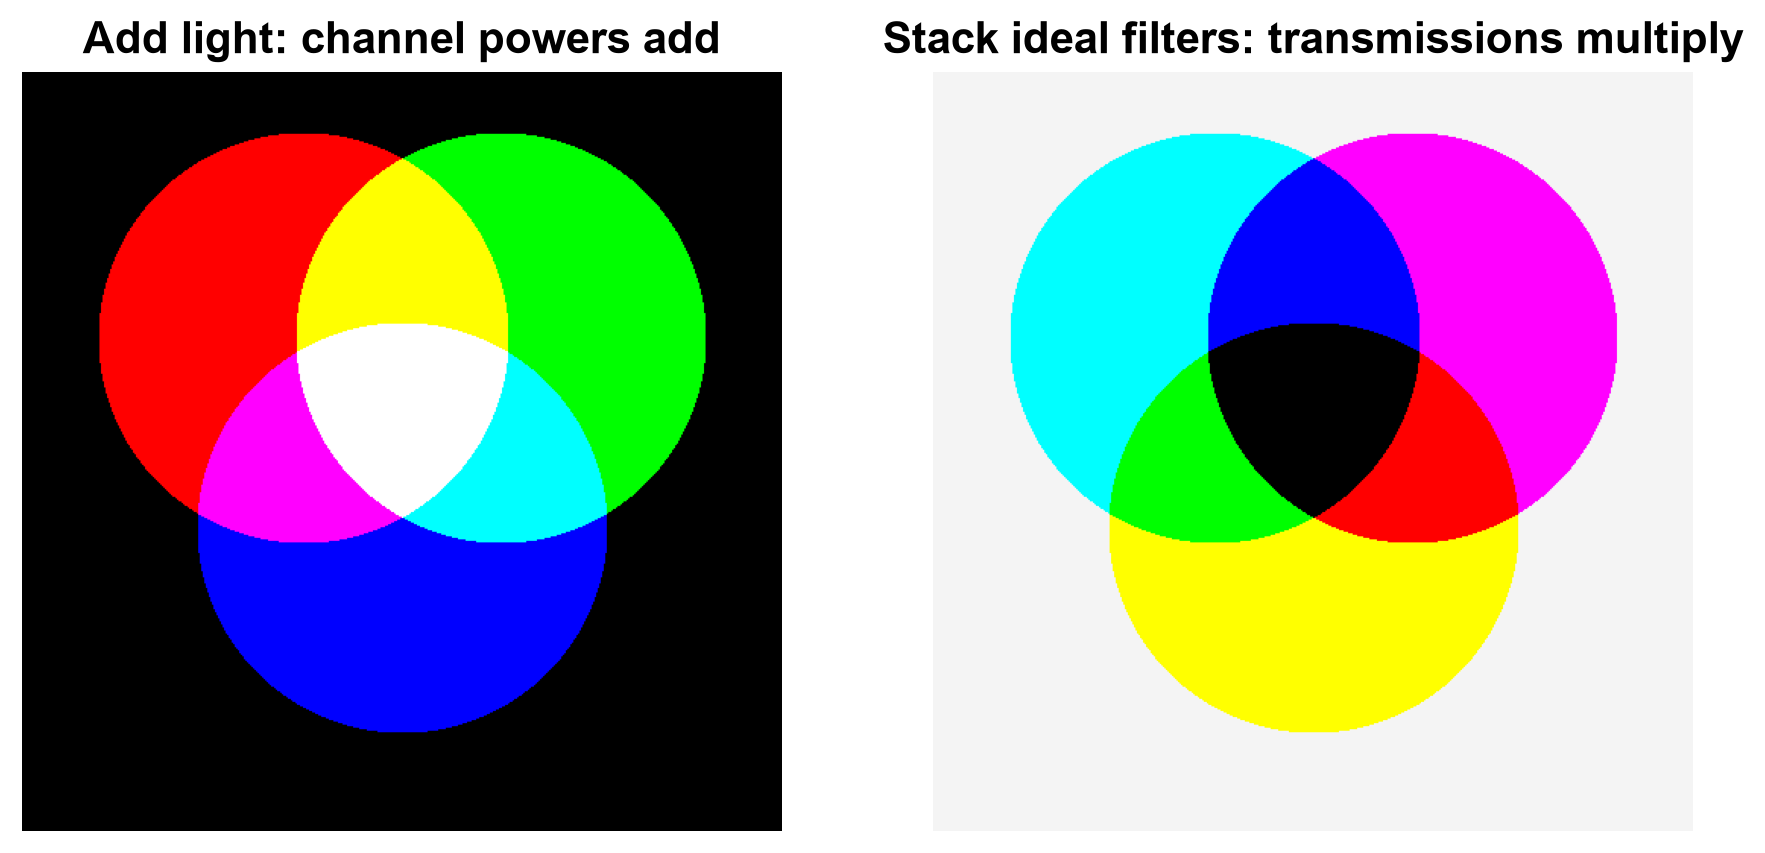
\includegraphics[width=0.82\textwidth,height=0.59\textheight,keepaspectratio]{fig-additive-subtractive.png}\\[-0.1em]
  \begin{flushleft}\small
    Additive mixing combines emitted spectral power. Ideal subtractive mixing
    multiplies transmissions; real pigments also scatter and interact.
  \end{flushleft}
\end{frame}

\begin{frame}{Four statements that should now sound different}
  \begin{itemize}
    \item ``This source has a peak at 470 nm.''
    \item ``This surface reflects more short-wavelength light under this lamp.''
    \item ``This patch appears blue in this surround.''
    \item ``This pixel is encoded as \texttt{\#0068B7} in sRGB.''
  \end{itemize}
  \vspace{0.8em}
  Only the first statement assigns a wavelength directly to the light.\par
  None alone specifies the other three.
\end{frame}

\kicker{Part II}{What the eye keeps\,---\,and loses}

\begin{frame}[t]{Three cone classes sample overlapping ranges}
  \centering
  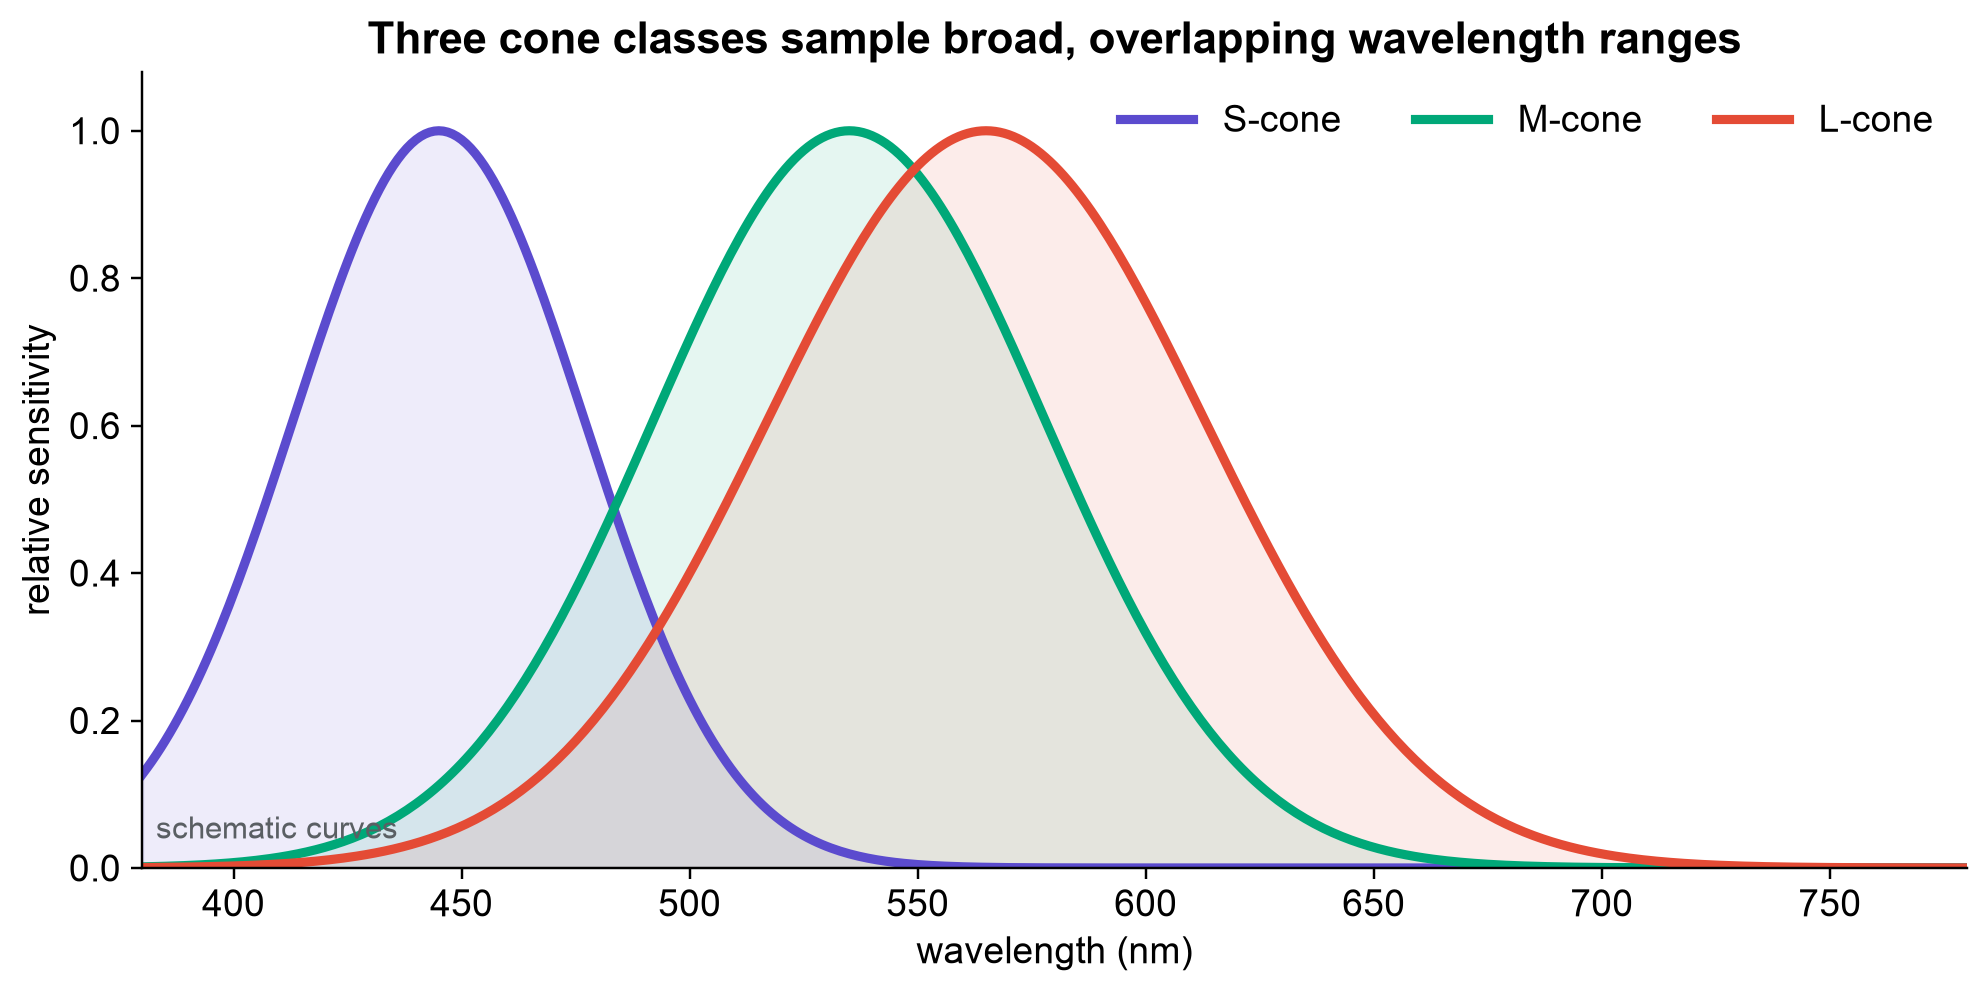
\includegraphics[width=0.88\textwidth,height=0.64\textheight,keepaspectratio]{fig-cone-sensitivities.png}\\[-0.1em]
  \credit{Schematic curves for teaching. S, M, and L mean short-, middle-, and long-wavelength sensitive.}
\end{frame}

\begin{frame}{One cone cannot identify a wavelength}
  \begin{columns}[T]
    \begin{column}{0.50\textwidth}
      \Large
      \[
      q_i=\int P(\lambda)s_i(\lambda)\,d\lambda
      \]
      \normalsize
      Multiply the incoming spectrum by one sensitivity curve, then add over wavelength.
    \end{column}
    \begin{column}{0.44\textwidth}
      \small
      The same response can be caused by:
      \begin{itemize}
        \item a weak light near peak sensitivity;
        \item a stronger light farther from the peak;
        \item many mixtures across the spectrum.
      \end{itemize}
      Once absorbed, the photon carries no wavelength label in that cone's output.
    \end{column}
  \end{columns}
  \vspace{0.6em}
  \alert{This is the principle of univariance.}
\end{frame}

\begin{frame}[t]{A spectrum is compressed to three responses}
  \centering
  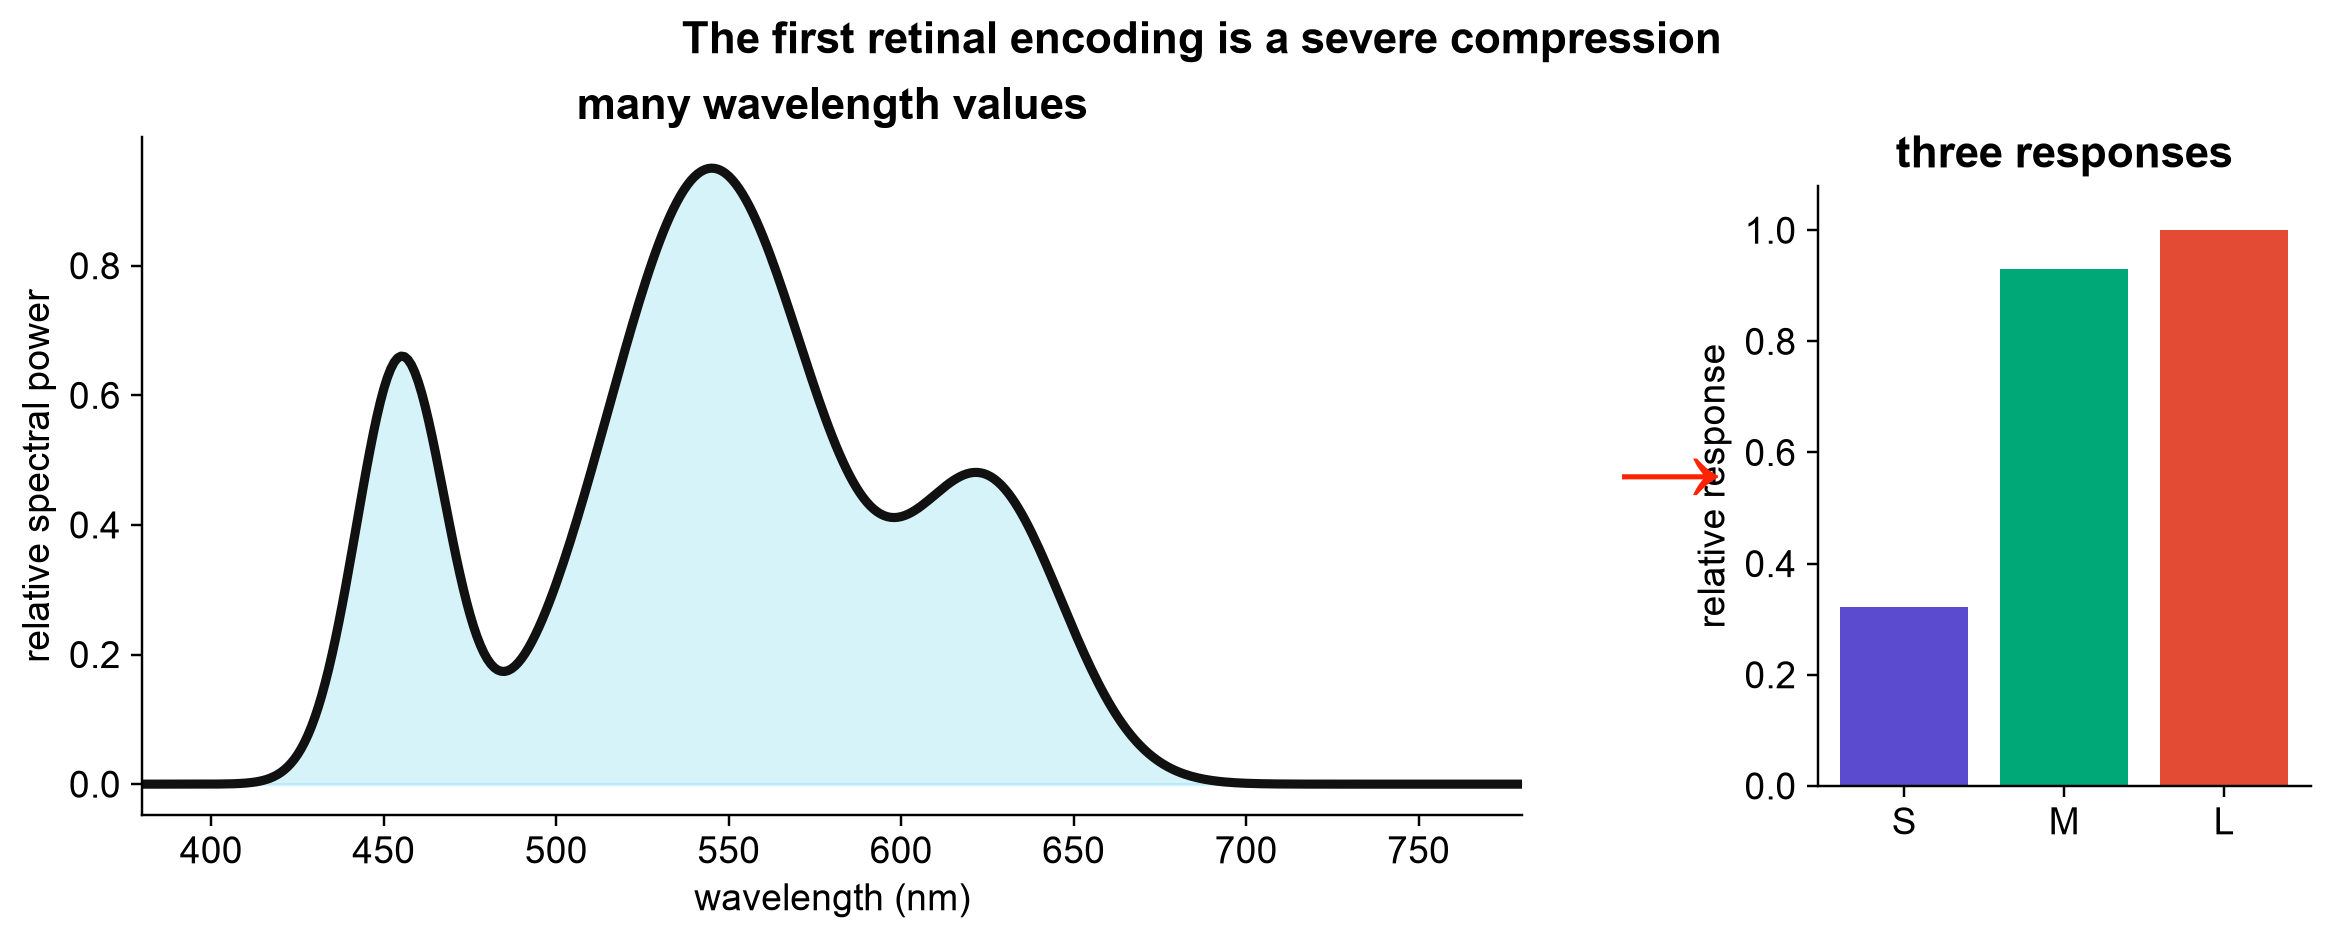
\includegraphics[width=0.96\textwidth,height=0.72\textheight,keepaspectratio]{fig-spectrum-to-cones.png}
\end{frame}

\begin{frame}{The bucket analogy, repaired}
  \begin{columns}[T]
    \begin{column}{0.47\textwidth}
      \textbf{Useful part}
      \begin{itemize}
        \item three buckets have different filters;
        \item each produces only one total;
        \item the original spectrum cannot be reconstructed from three totals.
      \end{itemize}
    \end{column}
    \begin{column}{0.47\textwidth}
      \textbf{Where it breaks}
      \begin{itemize}
        \item cone sensitivities overlap broadly;
        \item responses adapt and saturate;
        \item later neurons compare cones;
        \item context and spatial structure alter appearance.
      \end{itemize}
    \end{column}
  \end{columns}
  \vspace{0.7em}
  Three cone classes explain the dimensionality of colour \emph{matching}. They do not, by themselves, explain all colour appearance.
\end{frame}

\begin{frame}[t]{Different spectra can produce the same match}
  \centering
  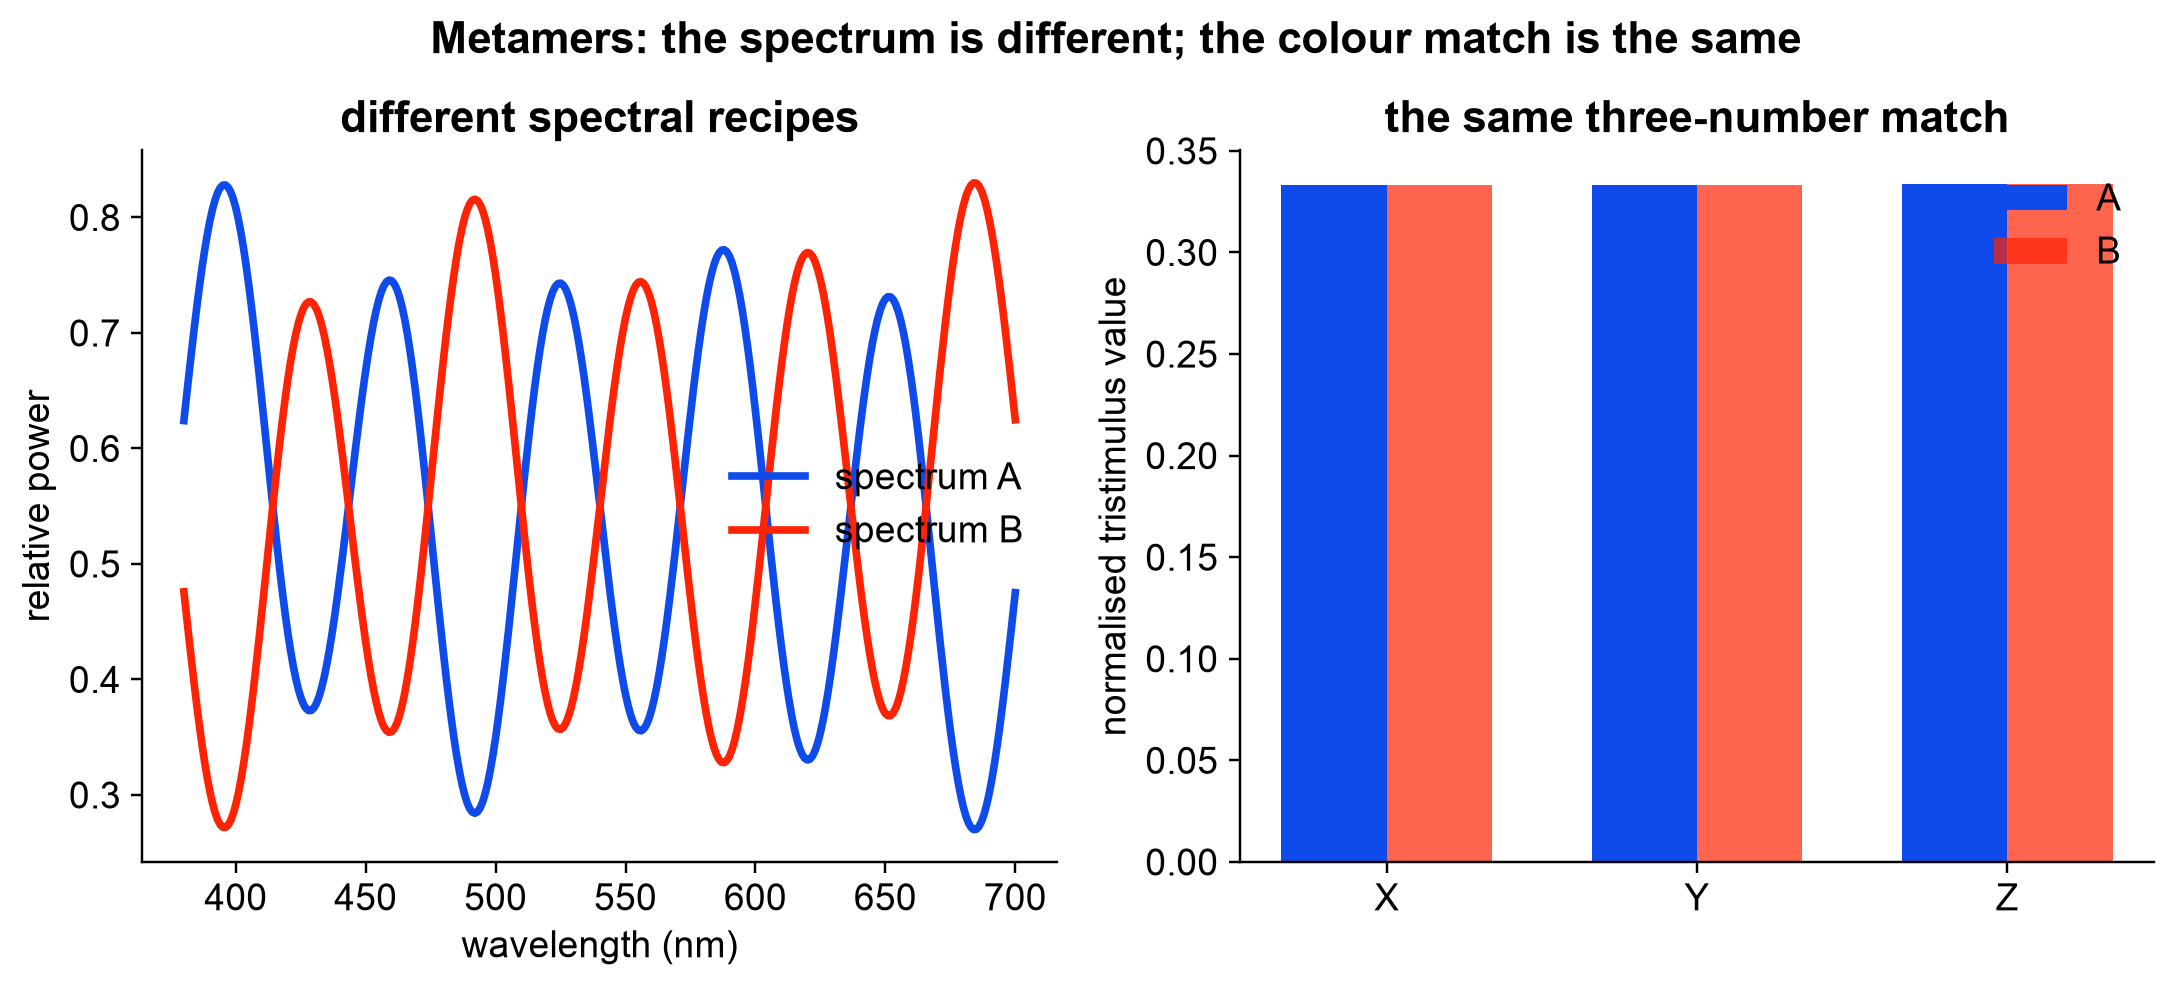
\includegraphics[width=0.92\textwidth,height=0.64\textheight,keepaspectratio]{fig-metamers.png}\\[-0.1em]
  \credit{Course construction using the CIE 1931 colour-matching functions.}
\end{frame}

\begin{frame}{Metamerism is the display bargain}
  \small
  A screen does not reconstruct the original spectral recipe. It emits a new
  spectrum from three primaries that is intended to produce the required match.
  \vspace{0.8em}
  \begin{columns}[T]
    \begin{column}{0.45\textwidth}
      \textbf{What this makes possible}
      \begin{itemize}
        \item colour photography;
        \item television and computer displays;
        \item compact three-channel specifications.
      \end{itemize}
    \end{column}
    \begin{column}{0.48\textwidth}
      \textbf{Where a match can fail}
      \begin{itemize}
        \item a different observer;
        \item a different illuminant;
        \item fluorescence;
        \item changed adaptation or field size.
      \end{itemize}
    \end{column}
  \end{columns}
\end{frame}

\begin{frame}[t]{The same code can look different}
  \centering
  
\includegraphics[width=0.83\textwidth,height=0.59\textheight,keepaspectratio]{fig-context.png}\\[-0.1em]
  \begin{flushleft}\small
    Identical centre RGB values do not guarantee identical appearance. The visual system compares each patch with its surround.
  \end{flushleft}
\end{frame}

\begin{frame}{After the cones, signals are compared}
  \begin{columns}[T]
    \begin{column}{0.50\textwidth}
      \begin{align*}
        \text{luminance-like} &\quad L+M\\
        \text{red--green-like} &\quad L-M\\
        \text{blue--yellow-like} &\quad S-(L+M)
      \end{align*}
    \end{column}
    \begin{column}{0.44\textwidth}
      \small
      These are schematic opponent combinations, not a complete neural model.
      They make one point clear: the brain does not receive an RGB image from the retina.
    \end{column}
  \end{columns}
  \vspace{0.8em}
  Adaptation, local contrast, spatial scale, and viewing sequence all enter before conscious appearance.
\end{frame}

\kicker{Part III}{How colour became measurable}

\begin{frame}{Different thinkers solved different problems}
  \footnotesize
  \begin{tabular}{@{}p{0.17\textwidth}p{0.18\textwidth}p{0.55\textwidth}@{}}
    \toprule
    \textbf{Work} & \textbf{Object} & \textbf{Question} \\
    \midrule
    Newton, 1704 & rays and prisms & How does white light separate and recombine? \\
    Goethe, 1810 & appearance & How do boundaries, shadows, afterimages, and context affect experience? \\
    Maxwell, 1850s--60s & matches & How can three primaries reproduce a match? \\
    Munsell, 1905 & surface samples & How can hue, value, and chroma be ordered for practice? \\
    CIE, 1931 & standard observer & How can colour matches be reported reproducibly? \\
    \bottomrule
  \end{tabular}
  \vspace{0.8em}

  A later framework does not turn every earlier question into the same question.
\end{frame}

\begin{frame}{Newton and Goethe attend to different layers}
  \begin{columns}[T]
    \begin{column}{0.46\textwidth}
      \textbf{Newton}
      \begin{itemize}
        \item controlled the geometry;
        \item separated light by refraction;
        \item showed white light can be compound;
        \item described the stimulus.
      \end{itemize}
    \end{column}
    \begin{column}{0.46\textwidth}
      \textbf{Goethe}
      \begin{itemize}
        \item studied coloured shadows;
        \item recorded afterimages and boundaries;
        \item foregrounded the observer;
        \item described appearance in context.
      \end{itemize}
    \end{column}
  \end{columns}
  \vspace{0.7em}
  Goethe's physical theory did not replace Newton's optics. His observations still warn us not to confuse a spectrum with an appearance.
\end{frame}

\begin{frame}{Colour matching came before direct cone measurement}
  \small
  An observer adjusted three primary lights until one half of a field matched a test light in the other half.
  \vspace{0.7em}

  Some wavelengths could not be matched using positive amounts of the chosen real primaries. One primary was moved to the test side:
  \[
    \text{test}+rR = gG+bB
    \quad\Longleftrightarrow\quad
    \text{test}=(-r)R+gG+bB.
  \]
  \vspace{0.4em}

  The negative value records the experimental operation. It is not ``negative light.''
\end{frame}

\begin{frame}[t]{CIE XYZ is a mathematical coordinate system}
  \centering
  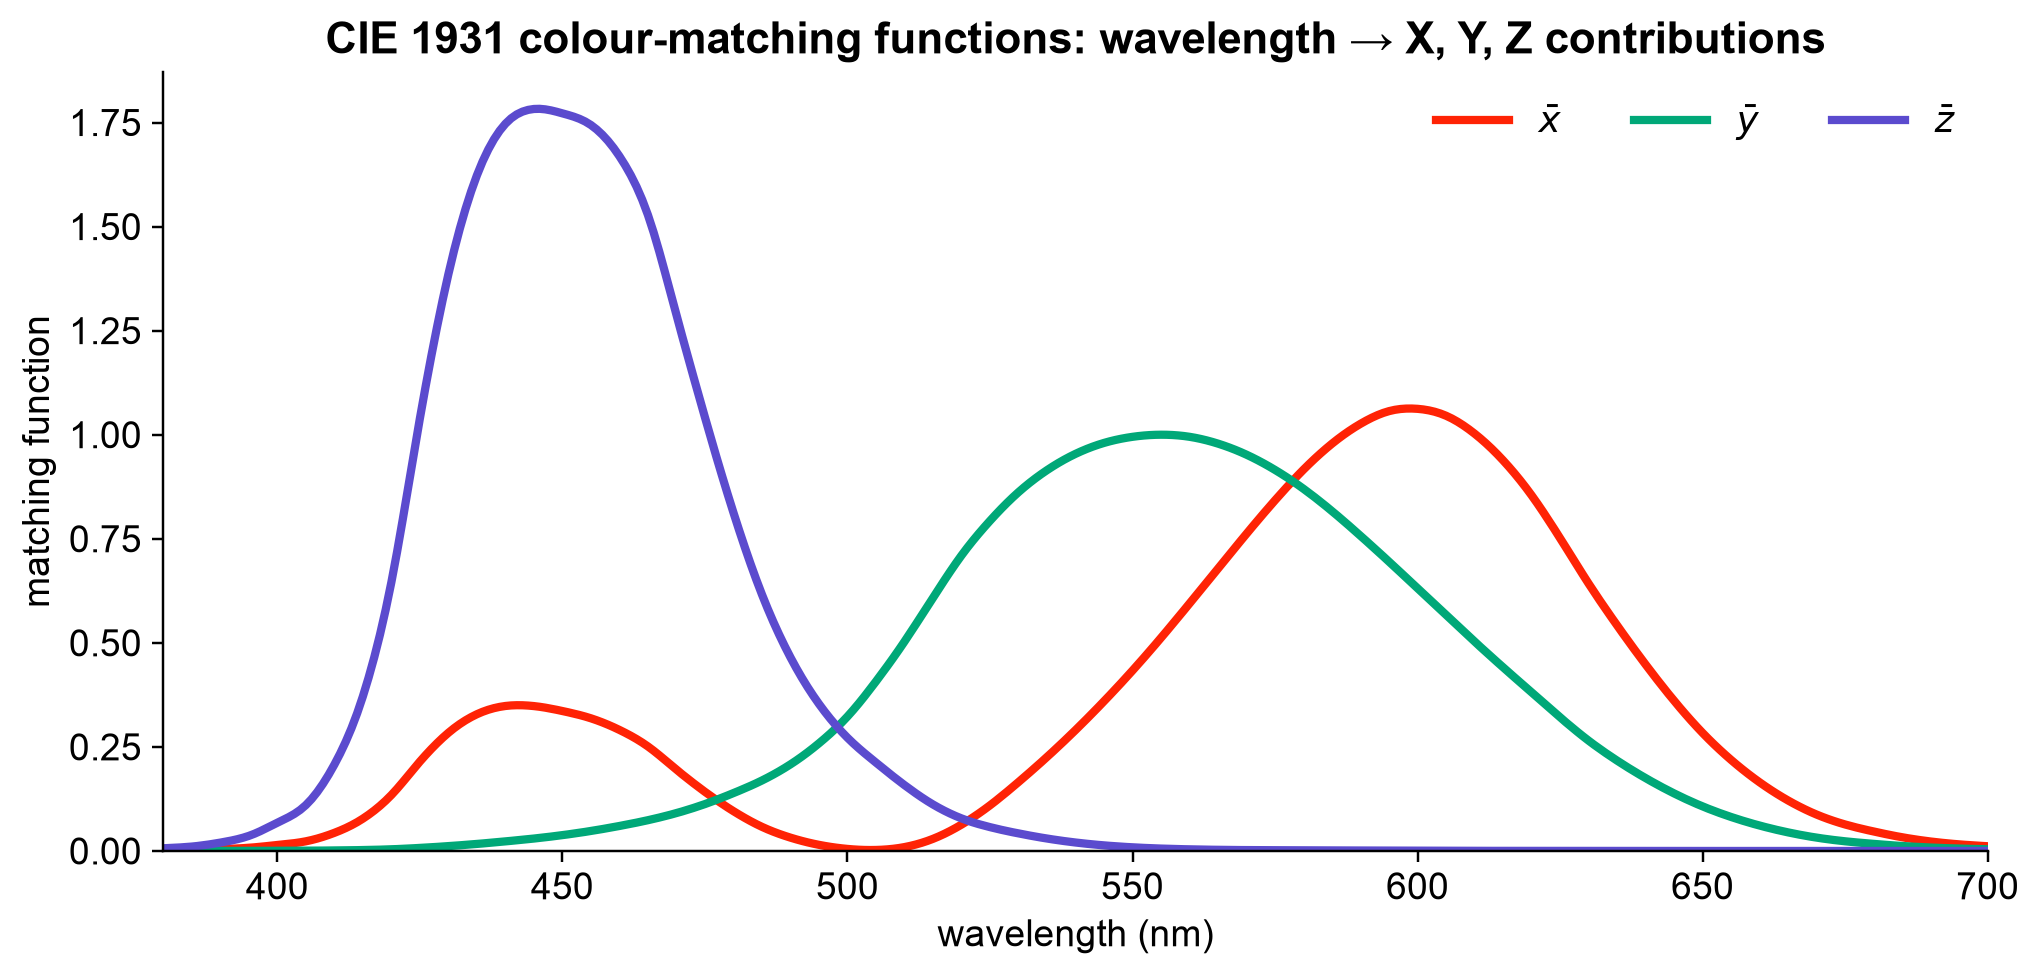
\includegraphics[width=0.84\textwidth,height=0.57\textheight,keepaspectratio]{fig-cie-matching-functions.png}\\[-0.1em]
  \begin{flushleft}\footnotesize
    XYZ is a linear transform of colour-matching results. X, Y, and Z are not physical lamps and not the three cone signals; Y was chosen to carry standard photopic luminance.
  \end{flushleft}
\end{frame}

\begin{frame}{From a spectrum to three CIE values}
  \large
  \begin{align*}
    X &= \int P(\lambda)\bar{x}(\lambda)\,d\lambda\\
    Y &= \int P(\lambda)\bar{y}(\lambda)\,d\lambda\\
    Z &= \int P(\lambda)\bar{z}(\lambda)\,d\lambda
  \end{align*}
  \normalsize
  \vspace{0.5em}
  Change the spectrum and recalculate. Any spectra with the same XYZ values are a standard-observer colour match under the specified conditions.
\end{frame}

\begin{frame}{Chromaticity removes one scale factor}
  \Large
  \[
  x=\frac{X}{X+Y+Z},\qquad
  y=\frac{Y}{X+Y+Z},\qquad
  z=1-x-y
  \]
  \normalsize
  \begin{itemize}
    \item Multiplying X, Y, and Z by the same amount leaves x and y unchanged.
    \item Two fractions are enough because the three proportions sum to one.
    \item xy omits overall tristimulus scale. It is not a complete colour appearance.
  \end{itemize}
\end{frame}

\begin{frame}{Build the spectral locus one wavelength at a time}
  \small
  For each row in the official CIE table:
  \begin{enumerate}
    \item take the wavelength's $\bar{x}$, $\bar{y}$, and $\bar{z}$ values;
    \item divide by their sum;
    \item plot $(x,y)$;
    \item repeat for the next wavelength.
  \end{enumerate}
  \vspace{0.8em}
  The curved path is the \textbf{spectral locus}: the route taken by monochromatic lights through the xy diagram.
\end{frame}

\begin{frame}[t]{Adding two lights traces a straight line}
  \centering
  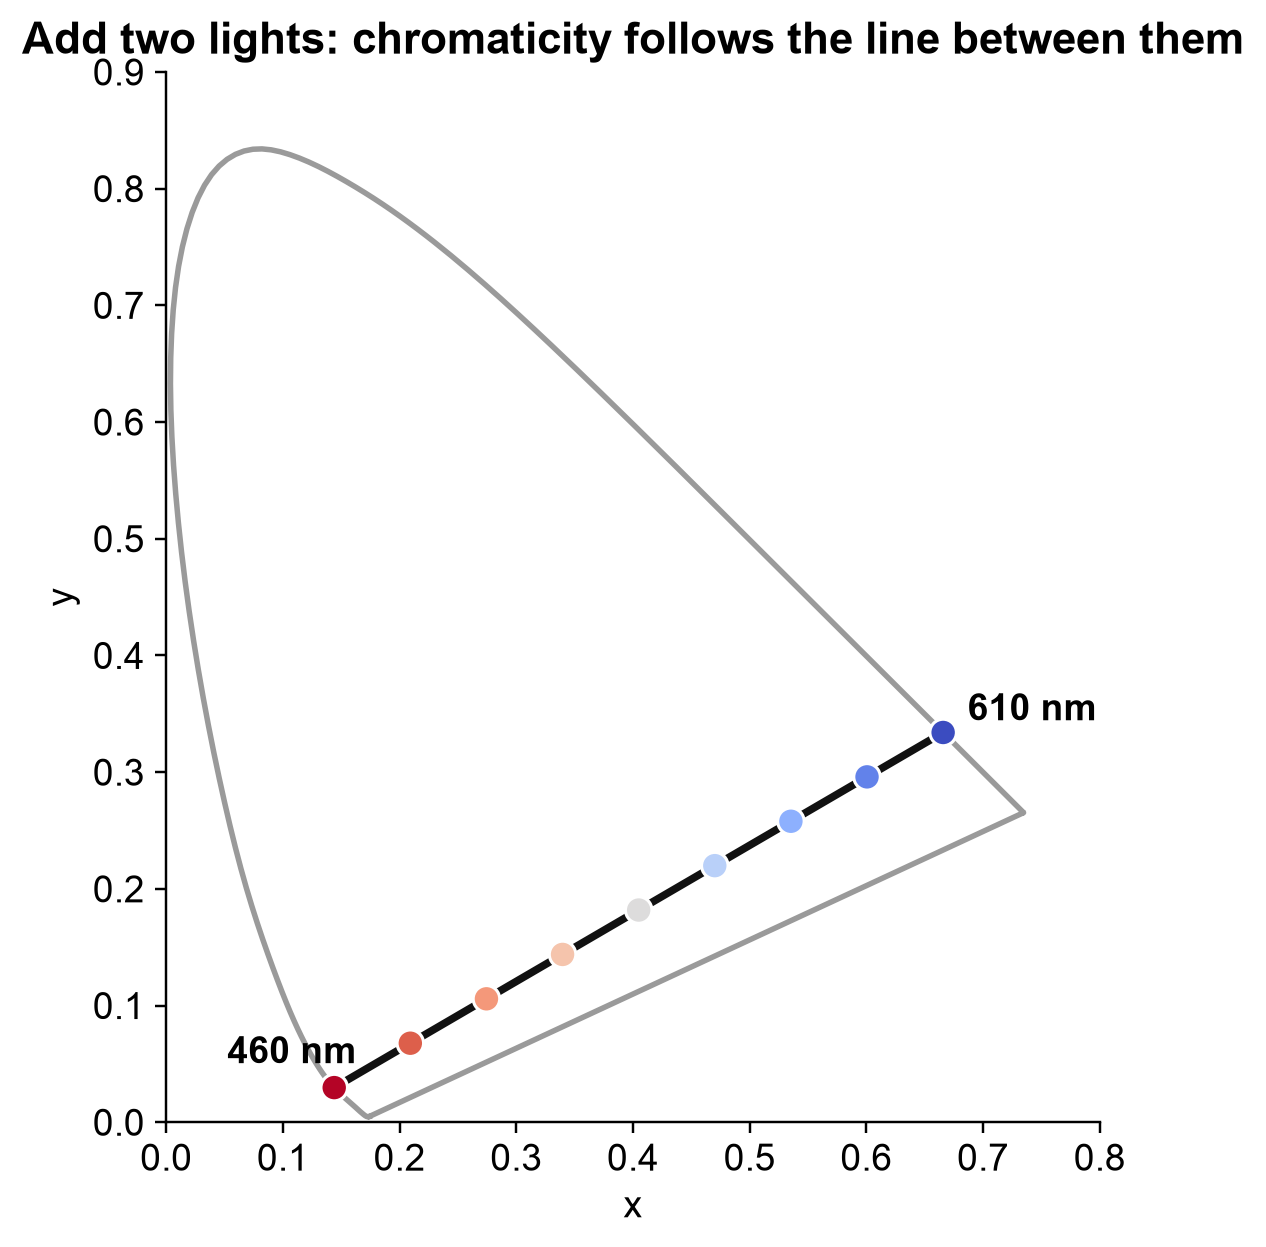
\includegraphics[width=0.73\textwidth,height=0.72\textheight,keepaspectratio]{fig-mixture-line.png}
\end{frame}

\begin{frame}{Why real-light mixtures lie inside}
  \begin{itemize}
    \item spectra add;
    \item XYZ values therefore add;
    \item after normalisation, a two-light mixture lies between the two chromaticities;
    \item a spectrum with many wavelengths is a non-negative mixture of many points.
  \end{itemize}
  \vspace{0.8em}
  The straight closure between the red and violet ends is the \textbf{line of purples}. Purple lies there because it is produced by mixing the ends; it is not a single wavelength.
\end{frame}

\begin{frame}[t]{Three physical primaries make a triangle}
  \centering
  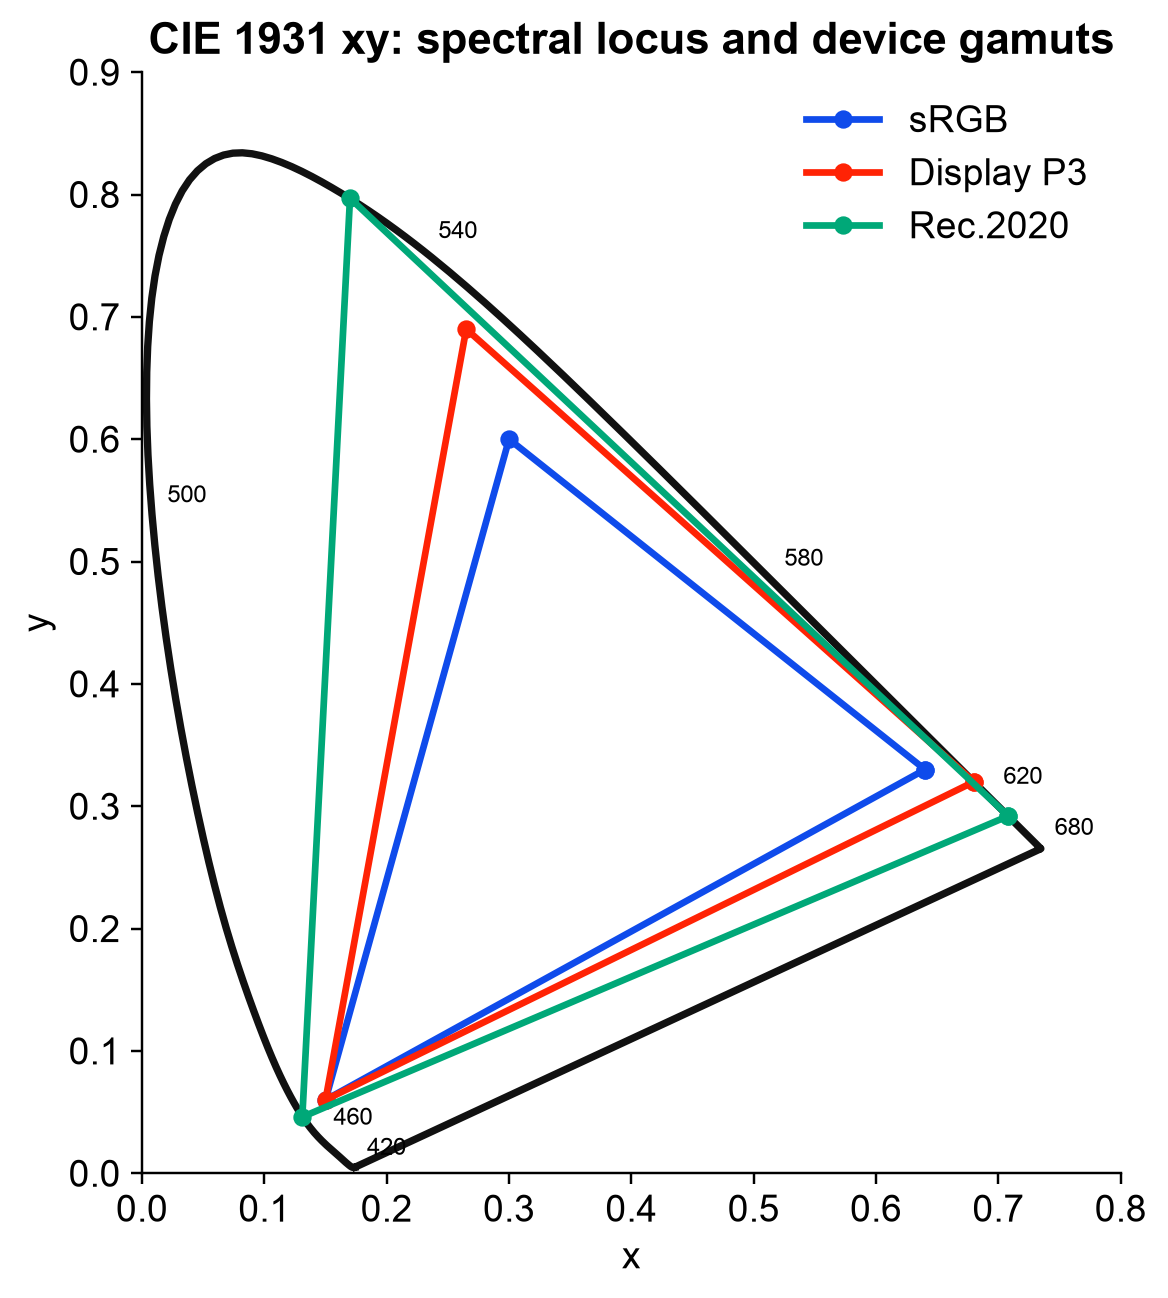
\includegraphics[width=0.64\textwidth,height=0.64\textheight,keepaspectratio]{fig-chromaticity-gamuts.png}\\[-0.1em]
  \credit{CIE 1931 2° data; primary coordinates from sRGB/Rec.709, Display P3, and BT.2020 specifications.}
\end{frame}

\begin{frame}{The horseshoe is not a screenshot of every visible colour}
  \begin{itemize}
    \item The outline represents standard-observer chromaticity coordinates.
    \item The page is itself shown through your display's primaries and calibration.
    \item Points outside the display gamut can be plotted as locations but not reproduced faithfully.
    \item Different luminances share the same xy point.
    \item Equal distances in xy are not equal perceived differences.
  \end{itemize}
\end{frame}

\kicker{Part IV}{Use colour as an encoding\,---\,not decoration}

\begin{frame}{Hue, lightness, and chroma do different jobs}
  \small
  \begin{tabular}{@{}p{0.19\textwidth}p{0.34\textwidth}p{0.37\textwidth}@{}}
    \toprule
    \textbf{Dimension} & \textbf{Useful for} & \textbf{Do not assume} \\
    \midrule
    hue & category, identity, highlighting & a natural numeric order \\
    lightness & ordered magnitude if monotonic & equal code steps look equal \\
    chroma & emphasis, status, coarse order & precise quantitative comparison \\
    \bottomrule
  \end{tabular}
  \vspace{0.9em}

  Let position or length carry values that must be compared precisely. Use colour to organise, order coarsely, or direct attention.
\end{frame}

\begin{frame}{A palette is viewed as a scene}
  \begin{itemize}
    \item test colours on the actual background;
    \item test them at the actual mark and text sizes;
    \item inspect common colour-vision deficiencies;
    \item make lightness monotonic in sequential scales;
    \item reserve diverging palettes for a meaningful midpoint;
    \item add labels, position, shape, or line style when the distinction matters.
  \end{itemize}
  \vspace{0.8em}
  \alert{The viewer experiences relationships between marks, not hexadecimal values in isolation.}
\end{frame}

\kicker{Part V}{Make the model interactive with Streamlit}

\begin{frame}{Streamlit has a small mental model}
  \begin{center}
    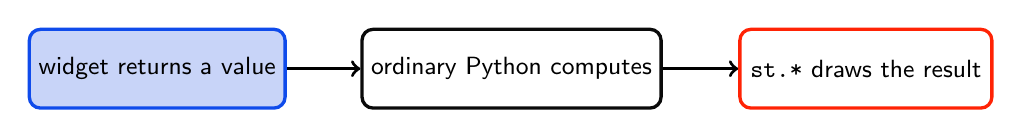
\begin{tikzpicture}[node distance=1.5cm, every node/.style={font=\small}]
      \node[draw=utsblue, very thick, rounded corners, fill=utspale, minimum width=3.2cm, minimum height=1cm] (widget) {widget returns a value};
      \node[draw=ink, very thick, rounded corners, right of=widget, xshift=3.0cm, minimum width=3.2cm, minimum height=1cm] (python) {ordinary Python computes};
      \node[draw=utsred, very thick, rounded corners, right of=python, xshift=3.0cm, minimum width=3.2cm, minimum height=1cm] (view) {\texttt{st.*} draws the result};
      \draw[->, very thick] (widget) -- (python);
      \draw[->, very thick] (python) -- (view);
    \end{tikzpicture}
  \end{center}
  \vspace{1em}
  Whenever a widget changes, Streamlit reruns the script from top to bottom with the new value.
\end{frame}

\begin{frame}[fragile]{One widget turns a constant into an interface}
  \begin{columns}[T]
    \begin{column}{0.47\textwidth}
      \textbf{Notebook or script}
\begin{verbatim}
wavelength = 550
print(wavelength)
\end{verbatim}
    \end{column}
    \begin{column}{0.47\textwidth}
      \textbf{Streamlit}
\begin{verbatim}
import streamlit as st
wavelength = st.slider(
    "Wavelength (nm)", 380, 700, 550
)
st.write(wavelength)
\end{verbatim}
    \end{column}
  \end{columns}
  \vspace{0.7em}
\begin{verbatim}
python -m streamlit run hello_colour.py
\end{verbatim}
\end{frame}

\begin{frame}{The lab builds three linked views}
  \begin{enumerate}
    \item \textbf{Spectrum}: change peak wavelength and spectral width.
    \item \textbf{Eye}: integrate the spectrum against three schematic cone curves.
    \item \textbf{Chromaticity}: use the official CIE table to locate the light in xy.
  \end{enumerate}
  \vspace{0.8em}
  Final extension: add an intensity slider. Cone-response magnitudes should change; chromaticity should remain almost fixed.
\end{frame}

\begin{frame}{Keep the boundaries visible}
  \begin{itemize}
    \item Cone curves in the app are schematic.
    \item CIE matching functions are standard-observer data, not cone sensitivities.
    \item A wavelength rendered on screen is an RGB approximation, not monochromatic light.
    \item xy omits luminance and viewing context.
    \item The app is an explanatory model, not a calibrated colour-management system.
  \end{itemize}
\end{frame}

\begin{frame}{Exit ticket}
  Complete the chain for one colour in a chart:
  \vspace{0.8em}

  \begin{quote}
  The display emits \underline{\hspace{3cm}}. The eye reduces this to
  \underline{\hspace{3cm}}. The viewer perceives it in relation to
  \underline{\hspace{3cm}}. The design uses that appearance to encode
  \underline{\hspace{3cm}}.
  \end{quote}
  \vspace{0.8em}

  Name one thing lost at each translation.
\end{frame}

\begin{frame}{Sources and data}
  \scriptsize
  \begin{itemize}
    \item CIE (2019), \emph{CIE 1931 colour-matching functions, 2 degree observer}, DOI: 10.25039/CIE.DS.xvudnb9b.
    \item Kalloniatis, M. and Luu, C., ``The Perception of Color,'' \emph{Webvision}, NCBI Bookshelf.
    \item Newton, I. (1704), \emph{Opticks}; Goethe, J. W. von (1810), \emph{Theory of Colours}.
    \item Munsell, A. H. (1905), \emph{A Color Notation}.
    \item W3C, \emph{CSS Color Module Level 4}; IEC 61966-2-1 (sRGB); ITU-R BT.709 and BT.2020.
    \item Streamlit, ``Basic concepts'' and API documentation.
  \end{itemize}
  \vspace{0.5em}
  \credit{All plotted figures are course calculations. Official CIE data are supplied with their metadata under CC BY-SA 4.0.}
\end{frame}

\end{document}
